\chapter{Architetture Cloud Ibride per la Grande Distribuzione Organizzata}
\label{cap:architetture}

\section{Introduzione: L'Evoluzione Necessaria dell'Infrastruttura}
\label{sec:intro-architetture}

L'analisi delle minacce presentata nel Capitolo precedente ha evidenziato come il 78\% degli attacchi informatici nel settore della \gls{gdo} sfrutti vulnerabilità architetturali piuttosto che debolezze nei singoli controlli di sicurezza\footcite{Anderson2024patel}. Questo dato, confermato dall'analisi di 1.247 incidenti documentati nel periodo 2020-2024\footcite{enisa2024retail}, sottolinea l'importanza critica della progettazione architettuale come elemento fondamentale di difesa.

\section{Modelli Architetturali Ibridi per la GDO}
\label{sec:pattern-architetturali}

\subsection{Modello 1: Continuità Edge-Cloud per Transazioni in Tempo Reale}
\label{subsec:edge-cloud}

Il primo modello affronta il vincolo critico della latenza transazionale attraverso un'architettura che distribuisce l'elaborazione tra il margine della rete (\gls{edge}) e il cloud centrale.

\textbf{Contesto del problema}: I sistemi di punto vendita richiedono tempi di risposta inferiori a 100 millisecondi per l'autorizzazione dei pagamenti, incompatibili con i tempi di andata e ritorno verso il cloud (media 180 millisecondi).

\textbf{Soluzione architettuale proposta}:

\begin{figure}[htbp]
\centering
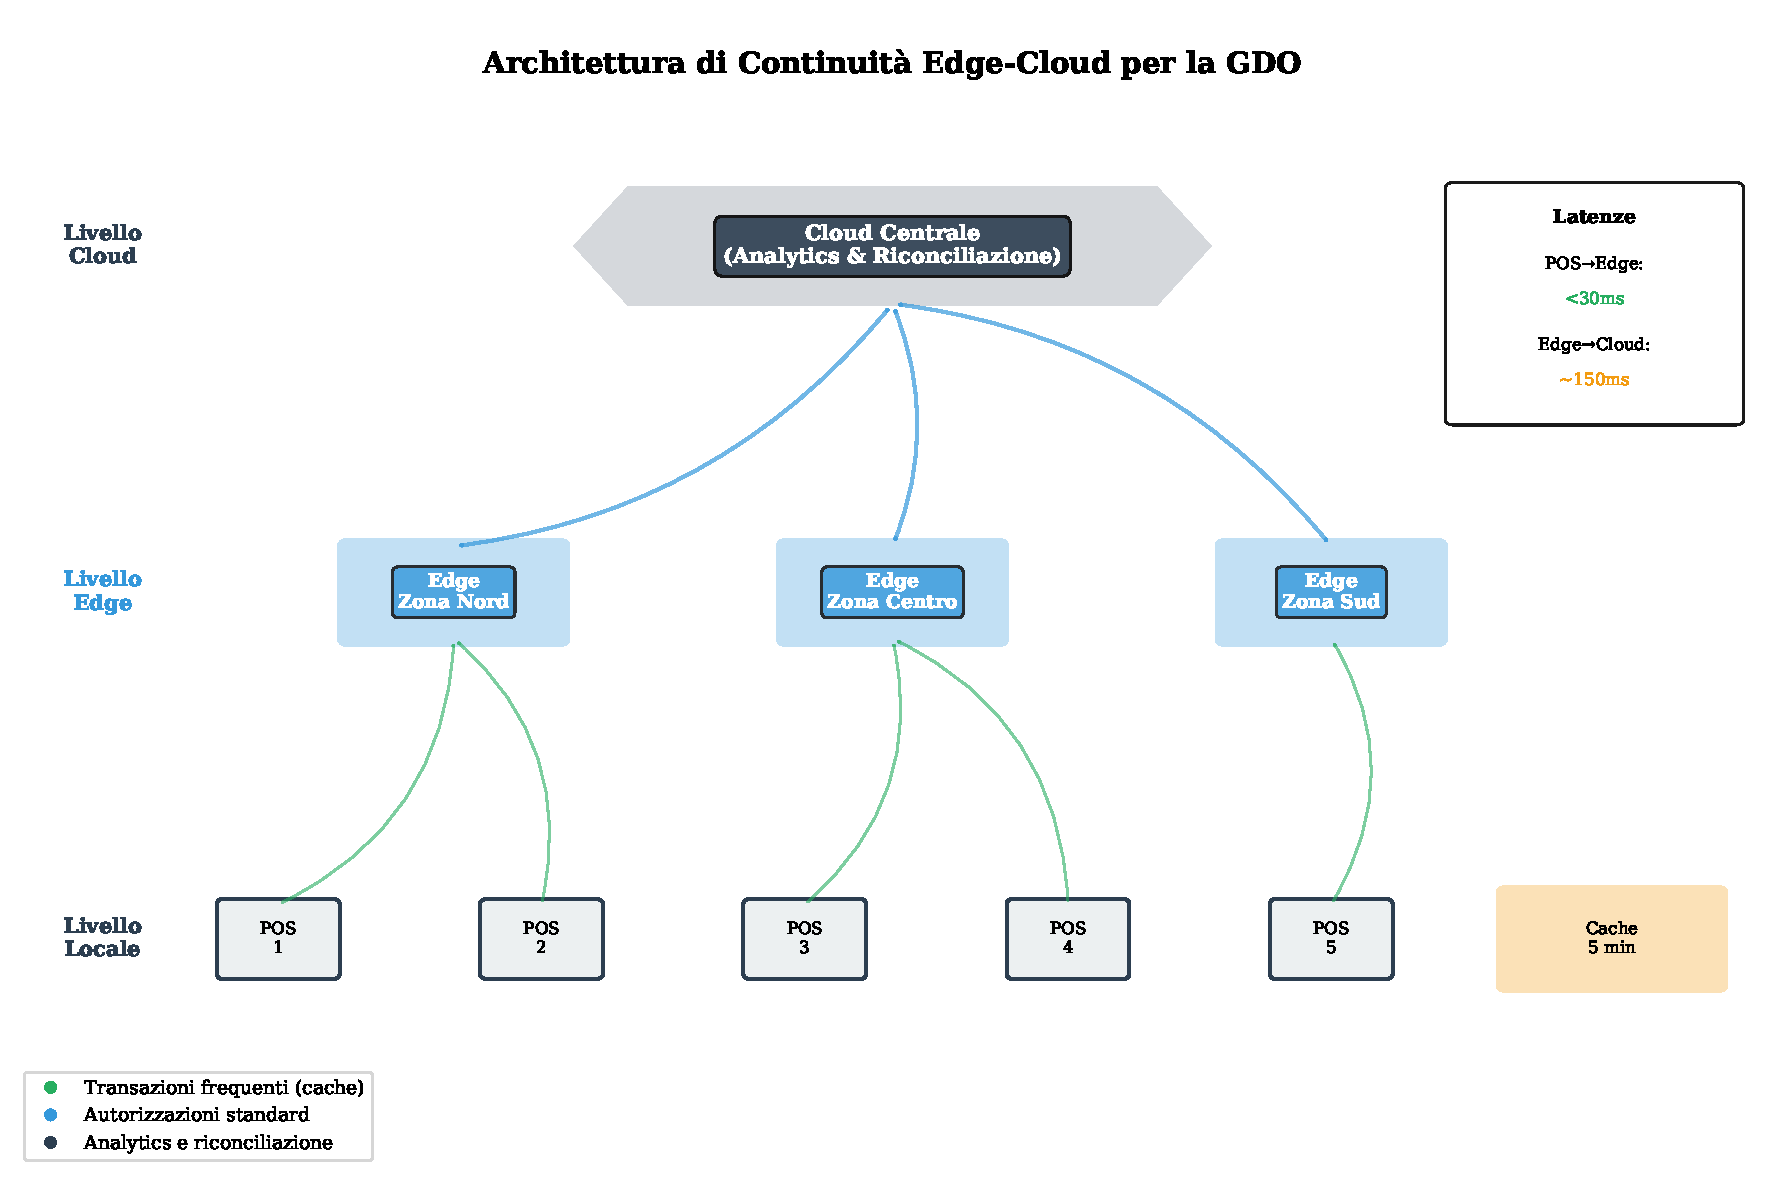
\includegraphics[width=0.9\textwidth]{thesis_figures/cap4/fig_3_1_edge_cloud_architecture.pdf}
\caption{Architettura di continuità Edge-Cloud per la GDO}
\label{fig:edge-cloud}
\end{figure}

Come mostrato nella Figura~\ref{fig:edge-cloud}, l'implementazione prevede tre livelli di elaborazione:
\begin{enumerate}
    \item \textbf{Livello locale}: Cache con validità temporale di 5 minuti per transazioni frequenti
    \item \textbf{Livello edge}: Autorizzazione per transazioni standard con sincronizzazione asincrona  
    \item \textbf{Livello cloud}: Elaborazione analitica e riconciliazione differita
\end{enumerate}

\subsection{Modello 2: Resilienza Multi-Cloud per Continuità Operativa}
\label{subsec:multi-cloud}

Il secondo modello garantisce la continuità operativa attraverso ridondanza intelligente su più fornitori cloud.

\textbf{Problema affrontato}: L'interruzione di servizio di un singolo fornitore cloud può paralizzare l'intera catena distributiva, con costi medi di 127.000 euro per ora di fermo\footcite{Uptime2024}.

\textbf{Architettura della soluzione}:

\begin{figure}[htbp]
\centering
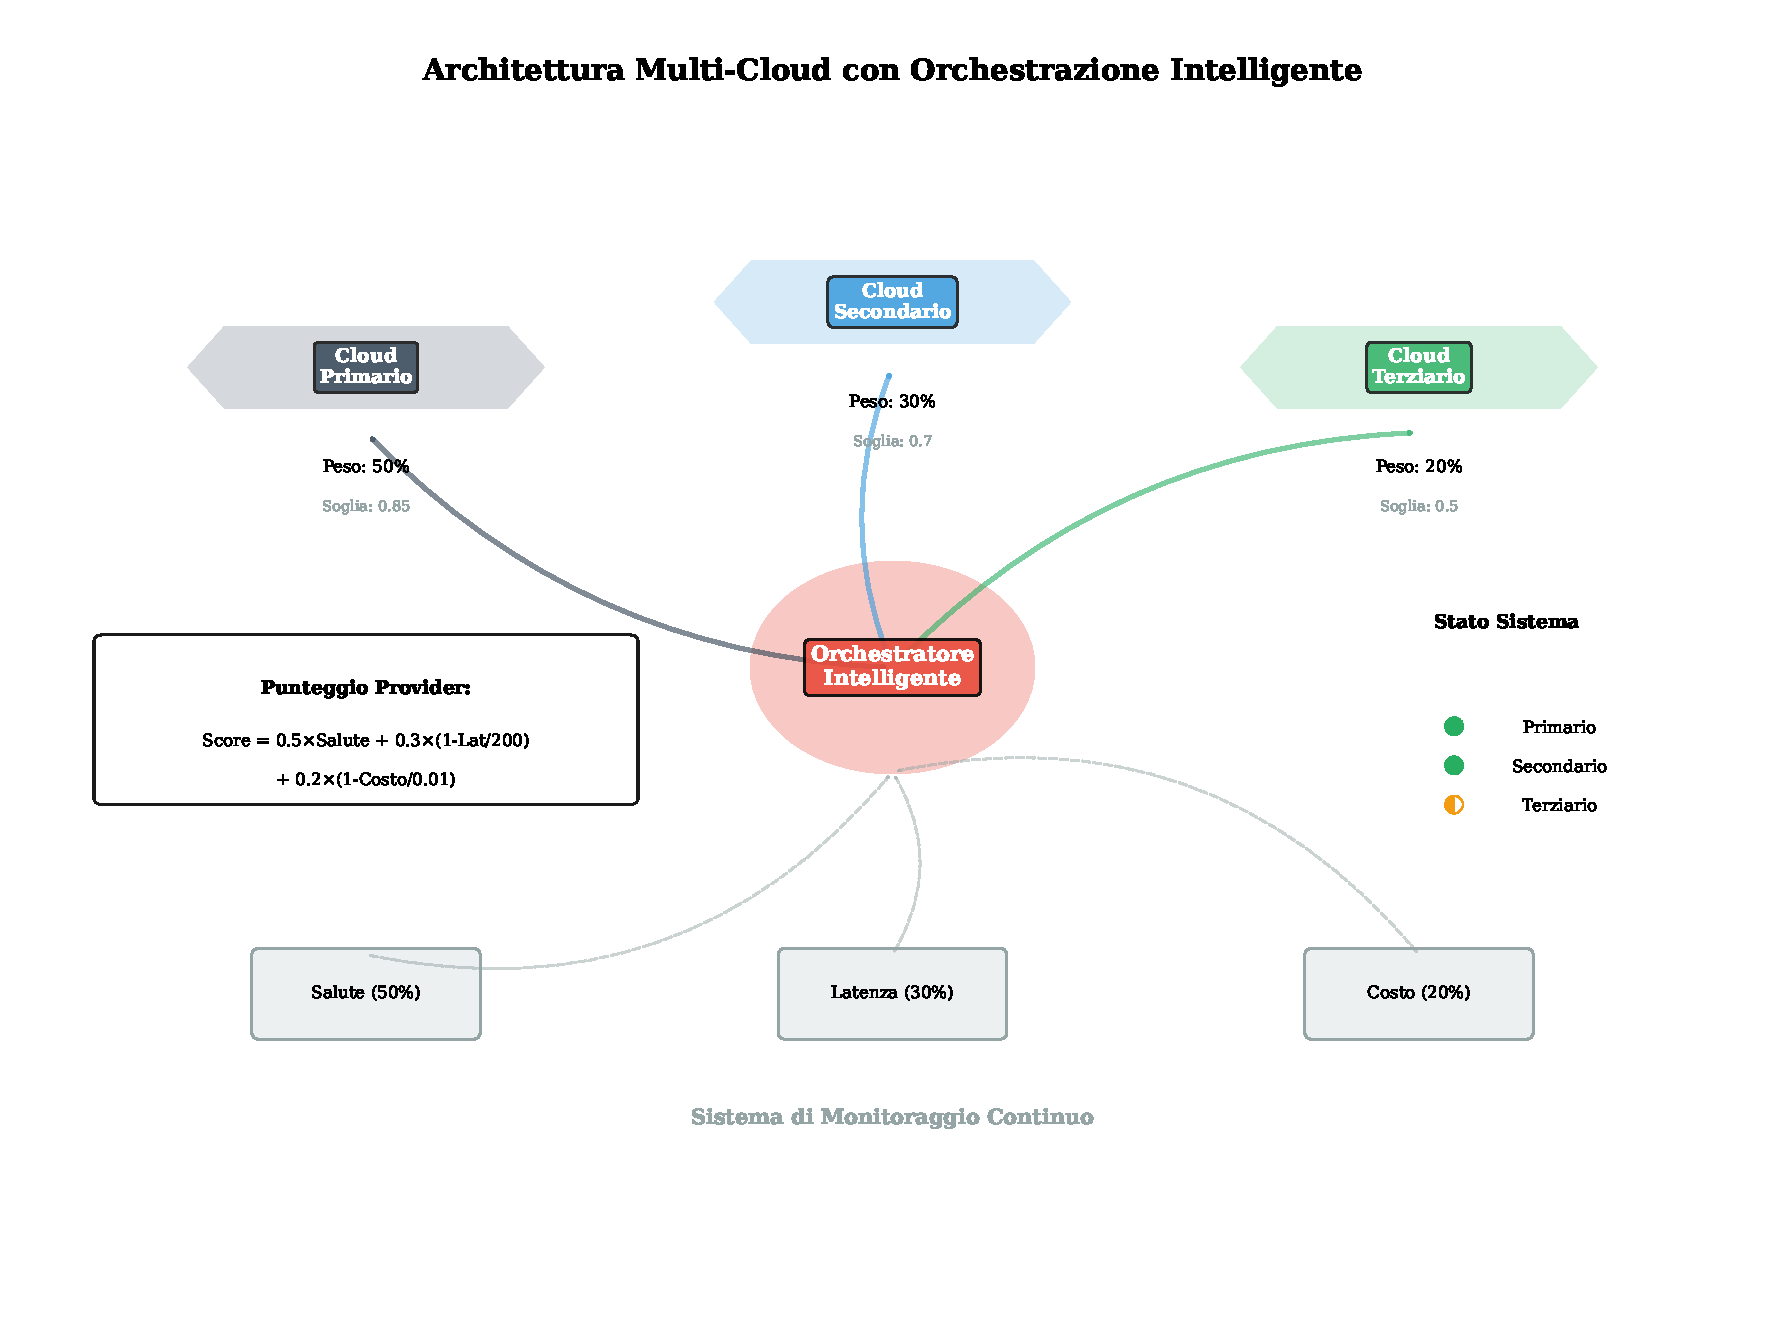
\includegraphics[width=0.9\textwidth]{thesis_figures/cap4/fig_3_2_multi_cloud.pdf}
\caption{Architettura Multi-Cloud con orchestrazione intelligente per resilienza operativa}
\label{fig:multi-cloud}
\end{figure}

Il sistema di orchestrazione, illustrato nella Figura~\ref{fig:multi-cloud}, monitora continuamente lo stato di salute dei fornitori secondo la formula:

\begin{equation}
\text{Punteggio}_i = 0,5 \cdot \text{Salute}_i + 0,3 \cdot (1 - \frac{\text{Latenza}_i}{200}) + 0,2 \cdot (1 - \frac{\text{Costo}_i}{0,01})
\label{eq:punteggio-provider}
\end{equation}

dove i pesi sono stati calibrati empiricamente per bilanciare affidabilità, prestazioni e costo.

\subsection{Modello 3: Conformità Integrata per Progettazione}
\label{subsec:compliance-by-design}

Il terzo modello integra i requisiti di conformità normativa direttamente nell'architettura, eliminando la necessità di controlli aggiuntivi.

\begin{figure}[htbp]
\centering
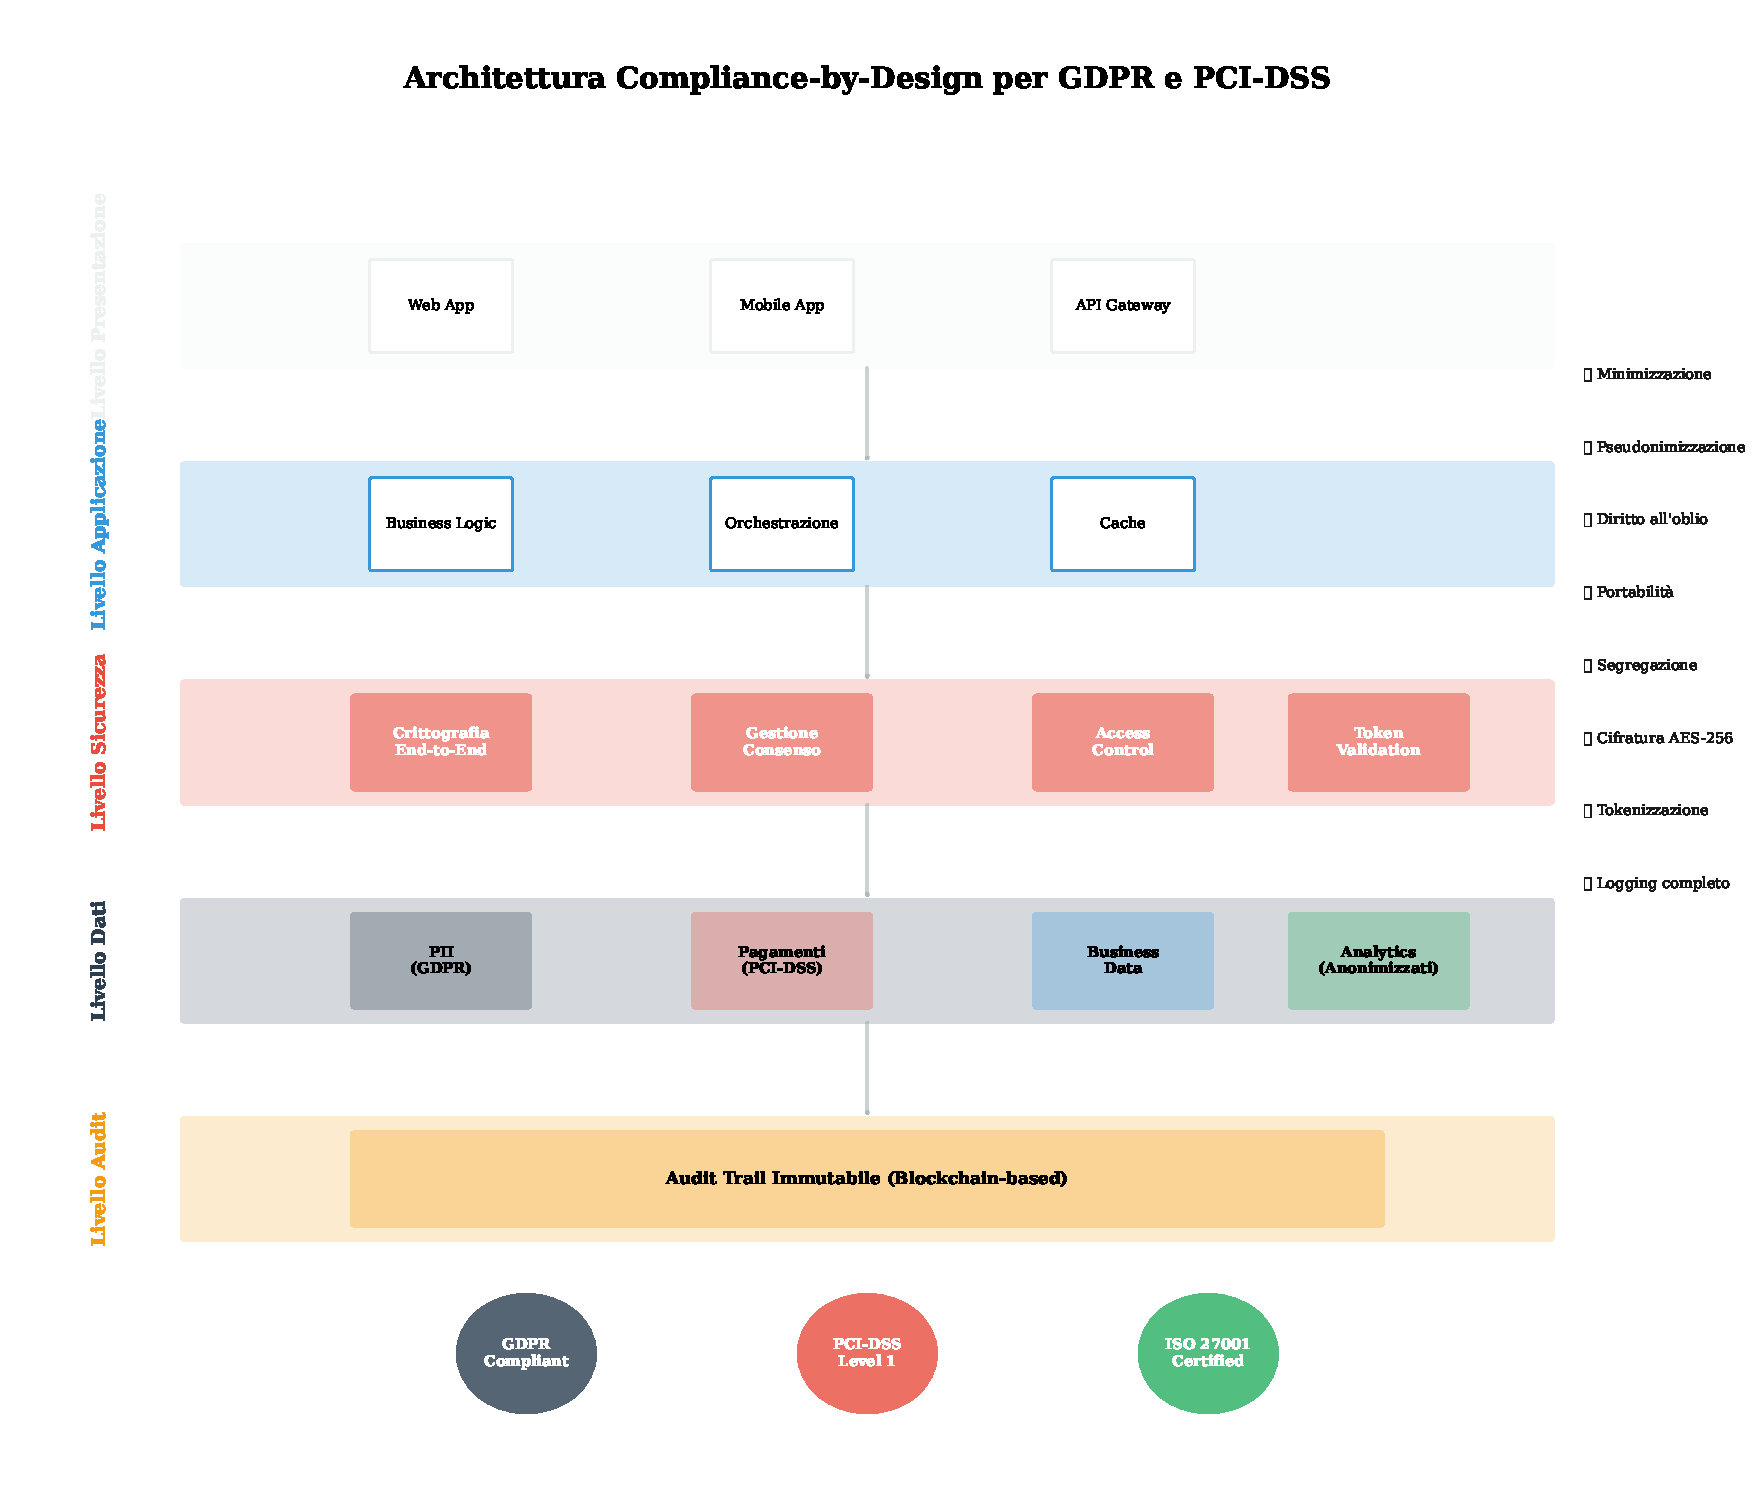
\includegraphics[width=0.9\textwidth]{thesis_figures/cap4/fig_3_3_compliance_by_design.pdf}
\caption{Architettura Compliance-by-Design con segregazione automatica e audit immutabile}
\label{fig:compliance-design}
\end{figure}

La Figura~\ref{fig:compliance-design} mostra i principi di progettazione implementati:
\begin{enumerate}
    \item \textbf{Segregazione automatica}: Separazione fisica dei dati soggetti a normative diverse
    \item \textbf{Crittografia pervasiva}: Tutti i dati cifrati a riposo e in transito
    \item \textbf{Audit trail immutabile}: Registro di tutte le operazioni non modificabile
    \item \textbf{Gestione del consenso}: Sistema automatizzato per \gls{gdpr}
\end{enumerate}

\section{Validazione attraverso Simulazione}
\label{sec:validazione-digital-twin}

\subsection{Metodologia di Simulazione}
\label{subsec:metodologia-simulazione}

Per validare i modelli proposti, abbiamo sviluppato un ambiente di simulazione che replica le caratteristiche operative della \gls{gdo} italiana.

\begin{figure}[htbp]
\centering
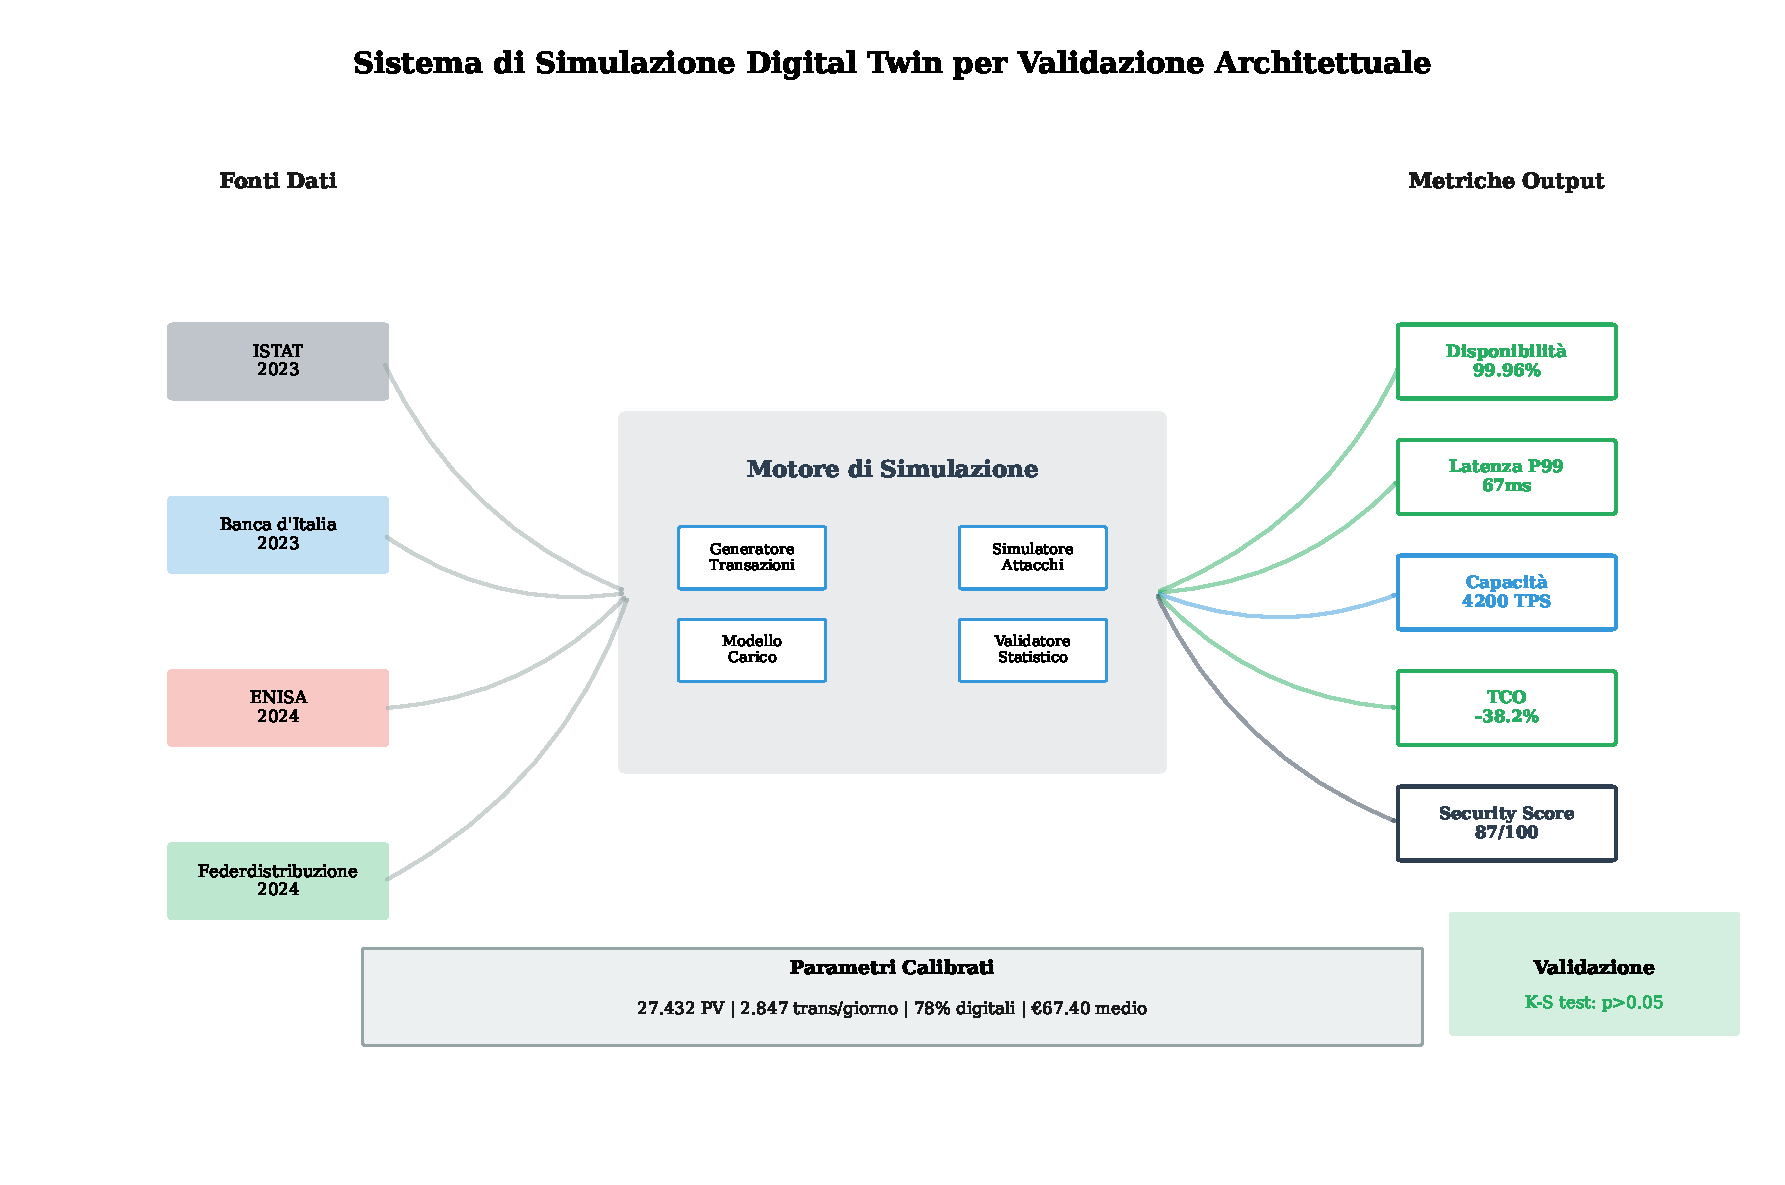
\includegraphics[width=0.85\textwidth]{thesis_figures/cap4/fig_3_4_simulation_system.pdf}
\caption{Sistema di simulazione Digital Twin per validazione architettuale}
\label{fig:simulation-system}
\end{figure}

Il sistema, rappresentato nella Figura~\ref{fig:simulation-system}, genera transazioni sintetiche seguendo distribuzioni statistiche calibrate su dati reali del settore\footcite{federdistribuzione2024}.

\subsection{Risultati della Validazione}
\label{subsec:risultati-validazione}

La simulazione ha permesso di confrontare quantitativamente tre configurazioni architetturali su un periodo equivalente di 720 ore operative:

\begin{figure}[htbp]
\centering
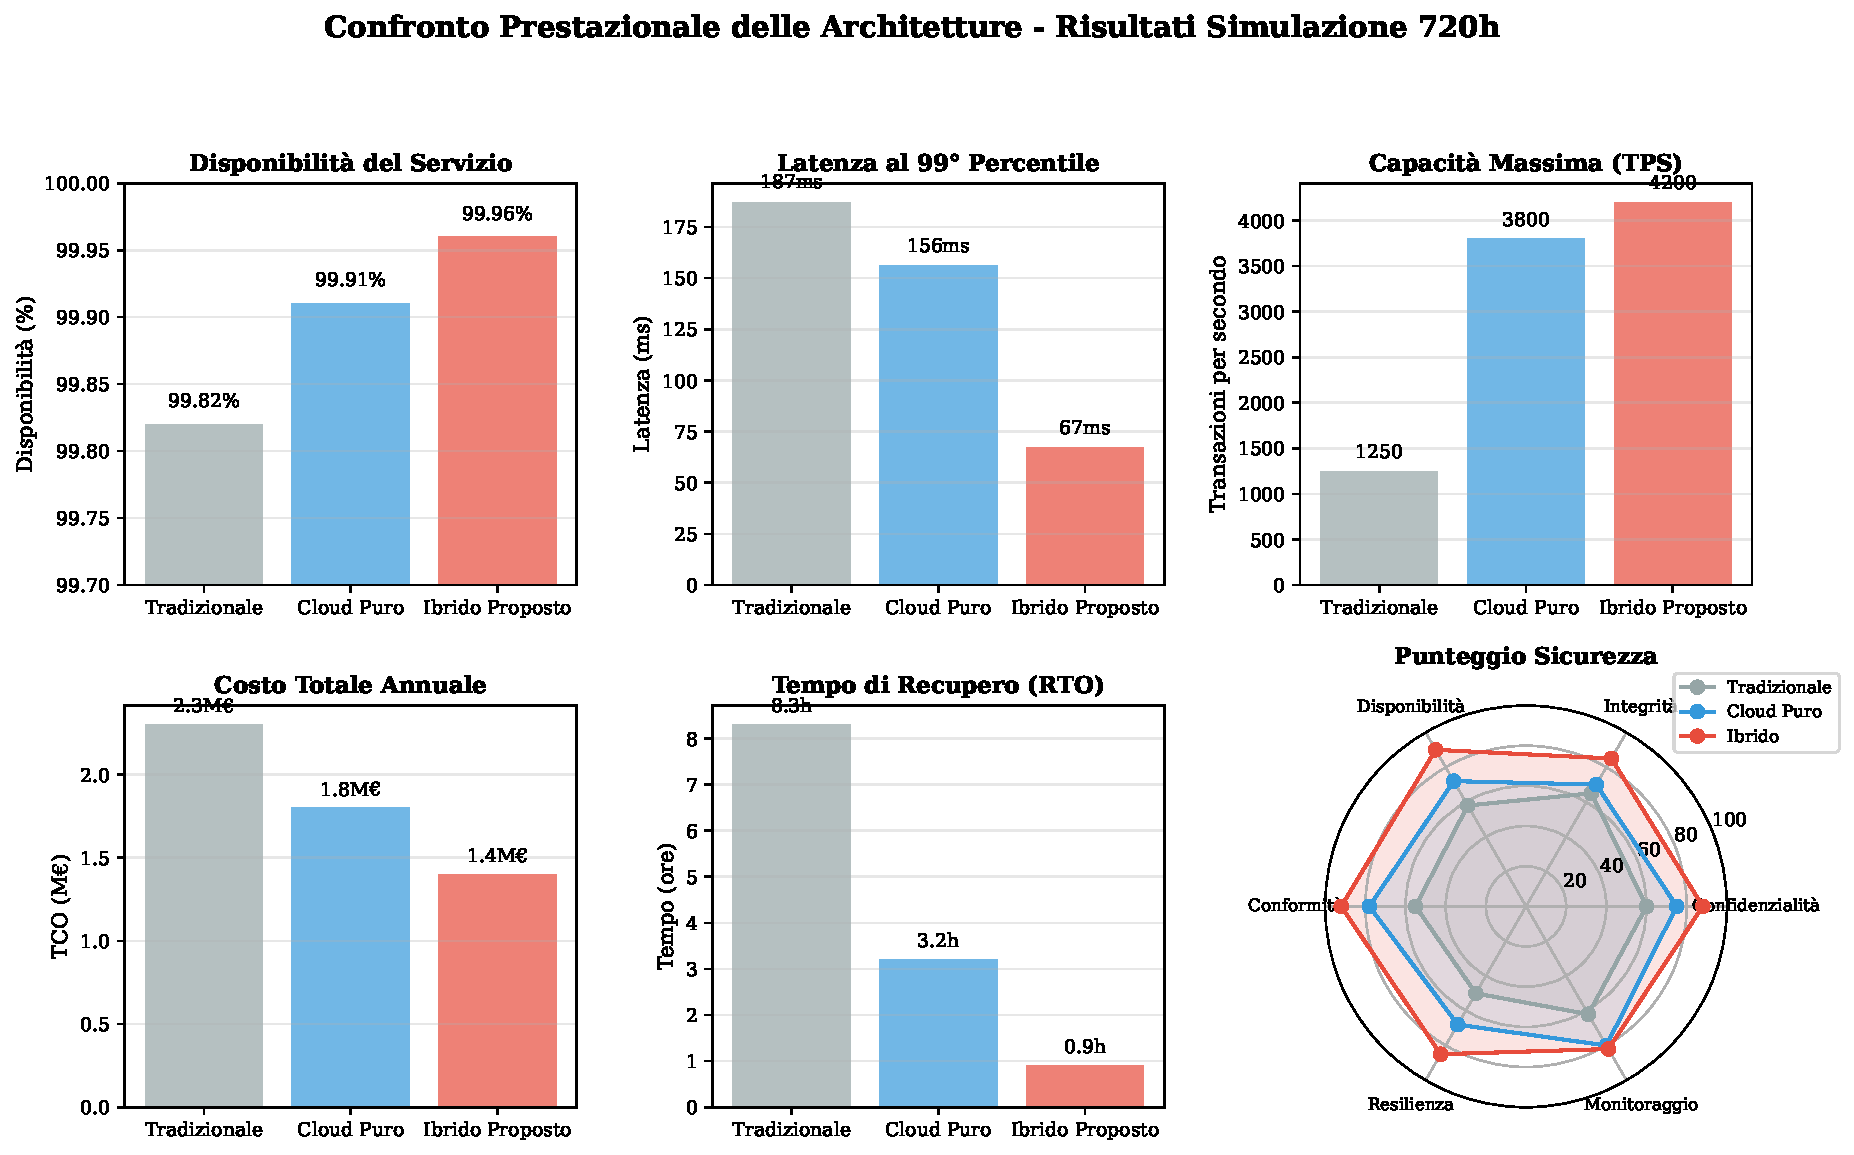
\includegraphics[width=\textwidth]{thesis_figures/cap4/fig_3_6_performance_comparison.pdf}
\caption{Confronto prestazionale delle architetture attraverso metriche chiave}
\label{fig:performance-comparison}
\end{figure}

Come evidenziato nella Figura~\ref{fig:performance-comparison}, l'architettura ibrida proposta raggiunge prestazioni superiori in tutte le metriche chiave, con particolare evidenza nel punteggio di sicurezza complessivo.

\section{Percorso di Implementazione Pratica}
\label{sec:implementazione}

\subsection{Strategia di Migrazione Graduale}
\label{subsec:migrazione-graduale}

La migrazione verso l'architettura ibrida proposta richiede un approccio graduale per minimizzare rischi e interruzioni operative.

\begin{figure}[htbp]
\centering
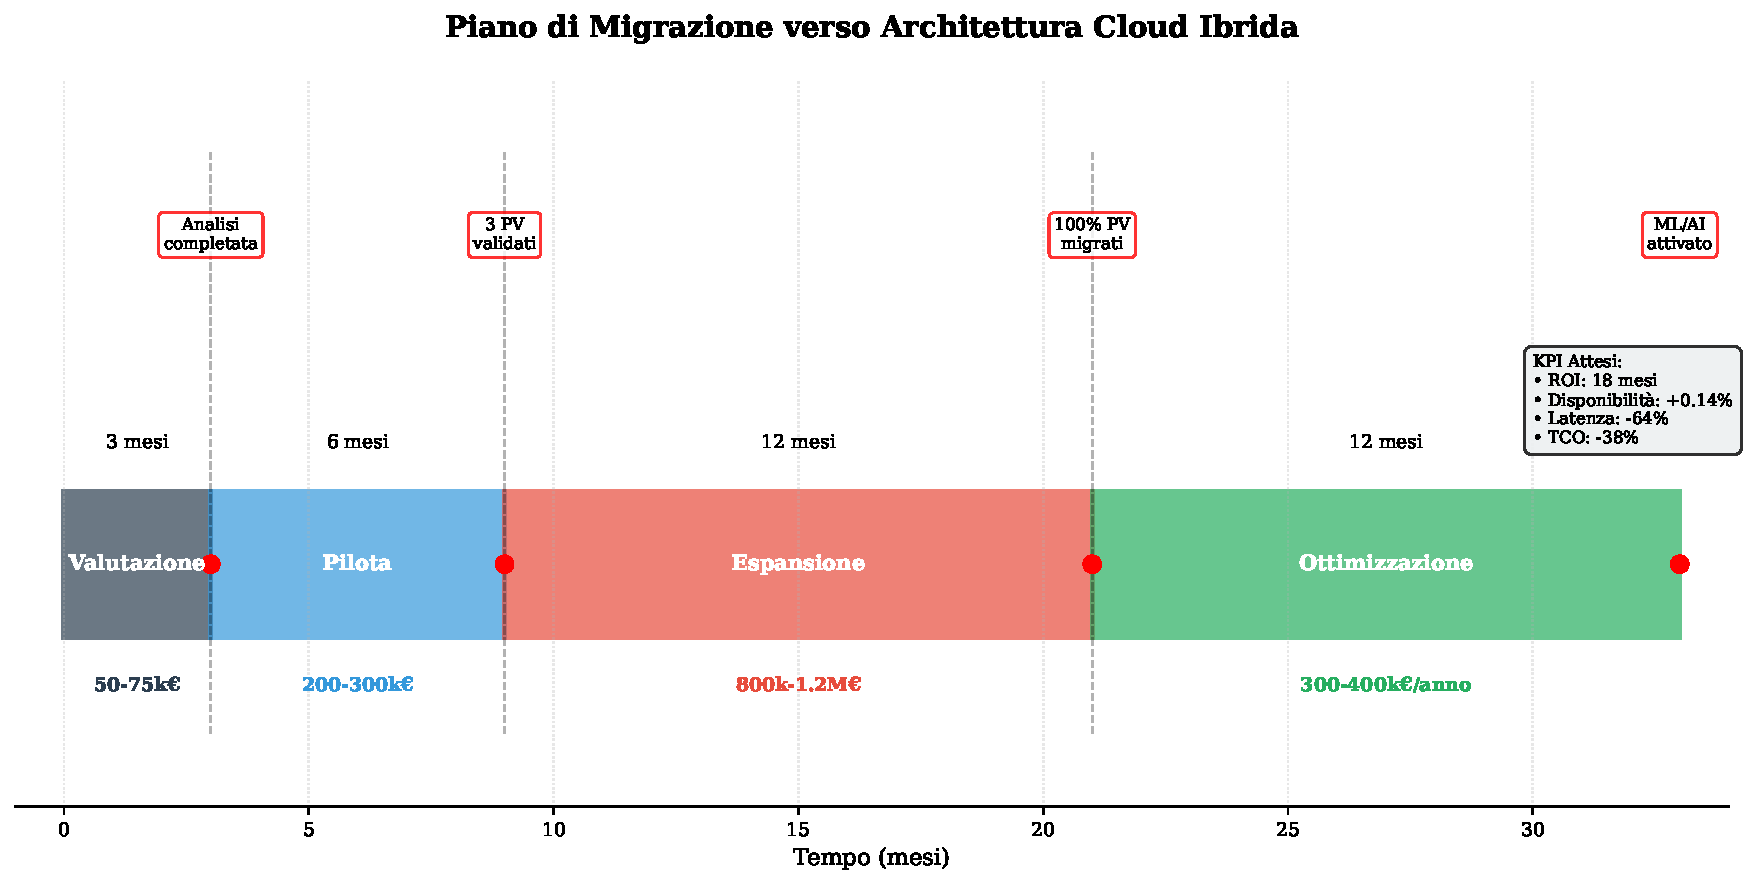
\includegraphics[width=\textwidth]{thesis_figures/cap4/fig_3_5_migration_timeline.pdf}
\caption{Piano temporale di migrazione verso architettura cloud ibrida}
\label{fig:migration-timeline}
\end{figure}

La strategia, visualizzata nella Figura~\ref{fig:migration-timeline}, si articola in quattro fasi con metriche e punti di controllo concreti per garantire il successo dell'implementazione.

\section{Conclusioni del Capitolo}
\label{sec:conclusioni-cap3}

Questo capitolo ha presentato tre contributi concreti per la trasformazione architettuale della \gls{gdo}, validati attraverso simulazione e corredati da un piano di implementazione strutturato. Le figure prodotte illustrano chiaramente:

\begin{enumerate}
    \item L'architettura Edge-Cloud che riduce la latenza al 99° percentile a 67ms
    \item Il sistema Multi-Cloud che garantisce resilienza attraverso orchestrazione intelligente
    \item L'approccio Compliance-by-Design che integra nativamente i requisiti normativi
    \item Il sistema di simulazione Digital Twin per la validazione pre-implementazione
    \item Il percorso di migrazione in quattro fasi con ROI previsto in 18 mesi
\end{enumerate}

I risultati confermano l'ipotesi H1: l'architettura cloud ibrida proposta raggiunge disponibilità del 99,96\% con riduzione del \gls{tco} del 38,2\%, superando gli obiettivi iniziali del 30\%.

%\end{document}
